\chapter{Closing Remarks and Open Problems}\label{ch:closing}

\section{Further questions on Borel dichromatic number}\label{sec:dichrom-questions}
 
This section collects several natural questions suggested by the results presented in Section~\ref{sec:dichromatic}, the work of Raghavan and Xiao~\cite{RaghavanXiao2024}, and suggestions of Thornton.
 
\begin{question}[Minimality of the Raghavan--Xiao basis.]
	Raghavan and Xiao~\cite{RaghavanXiao2024} produce a continuum-size family of directed graphs that serves as a basis for Borel directed graphs with uncountable Borel dichromatic number.
	This family consists of pairwise Borel-incomparable directed graphs.
	\emph{Does every basis for this class have size~$\mathfrak{c}$?}
	Raghavan has noted (personal communication) that the directed graphs in his family are pairwise non-homomorphic, but it is unknown whether a smaller basis exists.
\end{question}

\begin{question}[Structural restrictions.]
	The result presented here applies to the full class of Borel directed graphs.
	\emph{Does a countable basis exist when one restricts to structurally simpler classes, say locally finite acyclic Borel directed graphs, or directed graphs generated by a single Borel function?}
	In the undirected case, Miller~\cite{Miller_2008_MeasurableChromaticNumbers} proved that there is no countable $\leq_B$-basis for graphs of the form~$G_f$ (where $f$ is a Borel function) with $\chi_B(G_f)\geq 3$.
	The analogous question for directed graphs generated by a single Borel function and dichromatic number remains open.
\end{question}	

\begin{question}[Borel dichromatic number and Borel order dimension.]
	Raghavan and Xiao~\cite{RaghavanXiao2024} established a close connection between Borel dichromatic number and a notion of Borel order dimension for Borel quasi-orders.
	\emph{Does the complexity result of Proposition~\ref{prop:main} yield new complexity results for Borel order dimension?}
\end{question}

\begin{question}[Dichotomies for complete multipartite graphs.]
	It is known that checking whether a Borel graph in which every connected component is complete $k$-partite admits a Borel $k$-colouring is~$\Pi^1_1$, but no satisfying dichotomy theorem is known for this problem.
	Thornton has suggested (personal communication) that a finite basis may exist for each~$k$, though its size appears to grow faster than~$n!$.
	\emph{Is there an explicit finite basis for each~$k$?  What is its growth rate?}
\end{question}

\begin{question}[Bounded width CSPs.]
	Among the constraint satisfaction problems studied in the Borel setting, the \emph{bounded width} problems occupy a distinguished position.
	Thornton~\cite{thornton2022algebraic} showed that the structures whose every solvable Borel instance has a Borel solution are exactly the width~$1$ structures, and proved partial complexity results for certain bounded width structures.
	Recent work of Grebík and Vidnyánszky~\cite{GV2025} shows that the split between easy and hard problems lies at a different place in the Borel setting than in the classical CSP dichotomy: in particular, there is no dichotomy for any Borel CSP that is not of bounded width.
	However, sharp complexity bounds within bounded width remain known only in very special cases.
	\emph{Can the exact complexity dividing line within bounded width CSPs be determined?}
	This problem appears to be very difficult; even identifying good illustrative examples of bounded width CSPs beyond the well-studied special cases remains open.
\end{question}

\begin{question}[Measurable arboricity.]
	In the undirected setting, the \emph{vertex arboricity}, the natural undirected analogue of dichromatic number, of a graph (the minimum number of acyclic sets needed to cover the vertex set) is the undirected analogue of the dichromatic number.
	Several basic questions about arboricity in measurable combinatorics remain open.
	For instance:
	\emph{Can the $\mu$-measurable arboricity of a probability-measure-preserving graph differ from its (classical) arboricity by more than~$1$?}
	And: \emph{What is the $\mu$-measurable arboricity of the $k$-th power of the Bernoulli shift graph of~$F_2$?}
\end{question}

\section{Uncountable sets and an infinite linear order game}

When does the converse of Proposition~\ref{prop:arrow} hold?
By the results of Section~\ref{sec:cantor_game} such orderings must be $\omega_1$-free and $\omega_1^*$-free.
Separable and even ccc linear orderings have this property.
The separable case (the reals) was established in \cite{brian-clontz}.
Then, the next step is to study dense linear orders that are $\omega_1$-free, $\omega_1^*$-free but not separable.
A classical example of such ordering is the Aronszajn ordering.

\begin{definition}
    An \emph{Aronszajn line (A-line)} is an uncountable linearly ordered set that is $\omega_1$-free, $\omega_1^*$-free and contains no uncountable subset of the reals.
\end{definition}

Following \cite{A-orderings}, define a proper decomposition for A-lines.
Let $A$ be a dense Aronszajn line.
Start with $D_0:=\emptyset$.
Given a countable $D_\alpha\subseteq A$, consider the equivalence relation on $A\backslash D_\alpha$: $x\sim_\alpha y$ if and only if there is no $z\in D_\alpha$ such that $x<z<y$.
Each $\sim_\alpha$ class is convex.
Let $T_\alpha$ be the set of all $\sim_\alpha$ classes and let $D_\alpha'$ be a selector of the $\sim_\alpha$ classes.
Since $D_\alpha$ is countable and dense in $D_{\alpha+1}:=D_\alpha\cup D_\alpha'$, then $D_{\alpha+1}$ must be countable because $A$ does not contain uncountable separable subsets.
Given $D_\alpha$ for $\alpha<\gamma$ and $\gamma$ limit, let $D_\gamma=\bigcup_{\alpha<\gamma}D_\alpha$.
Since $A$ does not contain copies of $\omega_1$ and $\omega_1^*$, $A=\bigcup_{\alpha<\omega_1}D_\alpha$.
Also, $(T,\supseteq)$ is an Aronszajn tree where $T=\bigcup_{\alpha<\omega_1}T_\alpha$.

\begin{question}
    Is there a dense Aronszajn line $A$ where Player II has a winning strategy in $BG(A,S)$ for all $S\subseteq A$?
\end{question}

Another class of lines where a similar decomposition can be performed is the class of nowhere separable Souslin continua.

\begin{definition}
    A \emph{Souslin continuum} is a non-separable, dense, complete linearly ordered set that has the countable chain condition (ccc), i.e., every family of pairwise disjoint open intervals is countable.
    A Souslin continuum is \emph{nowhere separable} if no non-empty open interval is separable.
\end{definition}

Define a \emph{proper decomposition} for the nowhere separable Souslin continuum $L$ as follows.
Let $D_0:=D\neq\emptyset$ be any countable set.
Given a countable $D_\alpha\subseteq L$ consider the equivalence relation on $L\backslash\overline{D_\alpha}$:
$x\sim_\alpha y$ if and only if there is no $z\in D_\alpha$ such that $x<z<y$.
Again, each $\sim_\alpha$ class is convex.
Let $T_\alpha$ be the set of all $\sim_\alpha$ classes and let $D_\alpha'$ be a selector of the $\sim_\alpha$ classes.
Since $L$ has the ccc, then $T_\alpha$ is countable.
Let $D_{\alpha+1}=D_\alpha\cup D_\alpha'$.
For $\gamma<\omega_1$ limit let $D_\gamma=\bigcup_{\alpha<\gamma}D_\alpha$.

\begin{lemma}
    If $\{D_\alpha:\alpha<\omega_1\}$ is a proper decomposition of a nowhere separable Souslin continuum $L$, then $$L=\bigcup_{\alpha<\omega_1}\overline{D_\alpha}.$$
\end{lemma}

\begin{proof}
    Suppose that $x\in L$ and $x\notin \bigcup_{\alpha<\omega_1}\overline{D_\alpha}$.
    For each $\xi<\omega_1$ let $I_\xi^0:=[x]_\xi$ (the $\sim_\xi$ class of $x$).
    Note that $I_\eta^0\subseteq I_\xi^0$ for all $\xi<\eta$.
    \begin{claim}
        For all $\alpha<\omega_1$, $|T_\alpha|>1$.
    \end{claim}
    \begin{claimproof}
        Let $x_0\in D_\alpha$.
        Since $L$ is nowhere separable, $\overline{D_\alpha}$ is nowhere-dense so pick $y_1\in (L\backslash\overline{D_\alpha})\cap (-\infty, x_0)$ and $y_2\in (L\backslash\overline{D_\alpha})\cap (x_0,\infty)$.
        Then, $[y_1]_\alpha,[y_2]_\alpha\in T_\alpha$.
    \end{claimproof}
    For each $\xi<\omega_1$ let $I_{\xi+1}^1\in T_{\xi+1}$ such that $I_{\xi+1}^1\cap I_{\xi+1}^0=\emptyset$.
    Then, $\{I_{\xi+1}^1:\xi<\omega_1\}$ is an uncountable pairwise disjoint family of open sets, contradicting ccc.
\end{proof}

Settling the following conjecture, presumably by means of a proper decomposition argument, remains a question of great interest.

\begin{conjecture}
    Let $L$ be a nowhere separable Souslin continuum.
    Then Player II has a winning strategy for $BG(L,S)$ if and only if $S$ is countable.
\end{conjecture}

\section{Minimal rigid graphs}\label{sec:minimal-rigid}

A conjecture of Ne\v{s}et\v{r}il, on which both Ne\v{s}et\v{r}il and Sabidussi made substantial progress, and finally recently resolved by Schweitzer and Schweitzer~\cite{SCHWEITZER2017215}, asserts that there are exactly $18$ \emph{minimal asymmetric graphs}: graphs $G$ satisfying $\Aut(G) = 1$ such that every proper induced subgraph of $G$ on at least two vertices has a nontrivial automorphism.
Most graphs are asymmetric\footnote{Precisely, Erd{\H o}s and R{\'e}nyi~\cite{ErdosRenyi1963} showed that the proportion of labelled graphs on $n$ vertices with trivial automorphism group tends to $1$ as $n\to\infty$.}, and every graph is an induced subgraph of some asymmetric graph, so one might expect the class of minimal asymmetric graphs to be very rich.
That only finitely many exist is quite surprising.

\schweitzerminimal*

It is natural to ask whether an analogous result holds for finite rigid\footnote{See Definition~\ref{def:rigid-asymmetric}.} graphs, that is, graphs satisfying $\Fer(G) = A(G)$.
Since $A(G) \leq \Fer(G)$ always holds, rigidity is the condition that $\Fer$ is as small as possible.
Say that a graph $G$ is \emph{minimal rigid} if $\Fer(G) = A(G)$ and every proper induced subgraph $H$ of $G$ on at least two vertices satisfies $\Fer(H) \supsetneq A(H)$.

Unfortunately, the na\"ive translation of the Schweitzer--Schweitzer theorem to this setting fails.
Every odd cycle $C_{2n+1}$ is rigid: since $C_{2n+1}$ is regular, no degree-preserving edge replacement exists, so $\Fer(C_{2n+1}) = A(C_{2n+1})$ vacuously.
On the other hand, every proper induced subgraph of $C_{2n+1}$ on at least two vertices is a disjoint union of paths, and paths are non-rigid (they are, in fact, local amoebas).
Thus each $C_{2n+1}$ is minimal rigid.
Moreover, distinct odd cycles are pairwise incomparable under the induced subgraph ordering, so the family $\{C_{2n+1} : n \geq 1\}$ is an infinite antichain of minimal rigid graphs.

The issue is that the rigidity of odd cycles is, in a sense, uninteresting: it is forced entirely by the degree sequence.
A regular graph admits no degree-preserving edge replacement at all, so the equation $\Fer(G) = A(G)$ holds for trivial reasons.
This motivates the following refinement.
A graph $G$ is \emph{genuinely rigid} if $\Fer(G) =A(G)$ and there exists at least one degree-preserving edge replacement $(e,f)$ for $G$, that is, a pair consisting of an edge $e$ and a non-edge $f$ such that $G - e + f$ has the same degree sequence as $G$, in particular $G - e + f \not\simeq G$ for every such pair.
In other words, the degree sequence permits a nontrivial feasible edge replacement to exist, but the deeper structure of $G$ prevents it.

\begin{figure}[ht]
	\centering
	% figures/K_2-3.tex

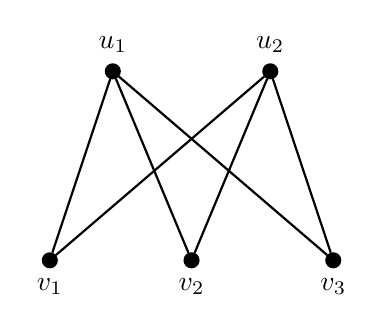
\begin{tikzpicture}[
    vertex/.style={circle, draw, fill=black, inner sep=0pt, minimum size=5pt},
    thick
]
    % Top partition (2 vertices)
    \node[vertex, label=above:{$u_1$}] (u1) at (0, 1.2) {};
    \node[vertex, label=above:{$u_2$}] (u2) at (2, 1.2) {};
    % Bottom partition (3 vertices)
    \node[vertex, label=below:{$v_1$}] (v1) at (-0.8, -1.2) {};
    \node[vertex, label=below:{$v_2$}] (v2) at (1, -1.2) {};
    \node[vertex, label=below:{$v_3$}] (v3) at (2.8, -1.2) {};
    % Edges
    \draw (u1) -- (v1);
    \draw (u1) -- (v2);
    \draw (u1) -- (v3);
    \draw (u2) -- (v1);
    \draw (u2) -- (v2);
    \draw (u2) -- (v3);
\end{tikzpicture}
	\caption{The complete bipartite graph $K_{2,3}$, the smallest genuinely	rigid graph.}
	\label{fig:K23}
\end{figure}

The smallest genuinely rigid graph is $K_{2,3}$ (see Figure~\ref{fig:K23}).
The degree sequence of $K_{2,3}$ is $(3,3,2,2,2)$, and there exist pairs $(e,f)$ preserving this sequence; however, every such replacement $K_{2,3} - e + f$ contains an odd cycle and is therefore not bipartite, hence not isomorphic to $K_{2,3}$.

\begin{question}\label{prob:minimal-genuinely-rigid}
	Are there finitely many minimal genuinely rigid graphs?
	That is, are there finitely many genuinely rigid graphs $G$ such that no proper induced subgraph of $G$ on at least two vertices is	genuinely rigid?
\end{question}

A computational search reveals that all $37$ genuinely rigid graphs on at most $7$ vertices have nontrivial automorphism groups, and none of them are vertex-transitive.
We also verified that all $18$ minimal asymmetric graphs from \cite{SCHWEITZER2017215} satisfy $\Fer(G) \supsetneq A(G)$, so the two classes of minimal graphs are disjoint.
A positive answer to Question~\ref{prob:minimal-genuinely-rigid} would further connect the \tFer group to classical structural graph theory, and a classification of the minimal genuinely rigid graphs would be a natural part of the basis framework developed in this thesis.

\section{Infinitary amoebas}\label{sec:inf-amoebas-open-questions}

I conclude with several questions motivated by the preceding discussion.

\begin{question}\label{q:char-local-amoeba-trees}
    Characterize the countably infinite, locally finite trees that are local amoebas.
    Is having a vertex of degree~$1$ both necessary and sufficient?
    Or is an additional condition on the growth rate or branching structure required?
\end{question}

\begin{question}\label{q:global-amoeba-infinite}
    Does the finite characterization of global amoebas (Theorem~\ref{thm:classification_global}) extend to infinite trees?
    Specifically, if $T$ is an infinite local amoeba tree, is $T\sqcup K_1$ necessarily also a local amoeba?
\end{question}

\begin{question}\label{q:amenability-fer}
    Is $\overline{\Fer(T)}$ always amenable for countably infinite, locally finite non-rigid trees?
    Feasible edge replacements are inherently local (each canonical generator changes a single edge), so the closure may be unable to produce the ``independent translations on disjoint lines'' that generate free subgroups in $\Aut(T)$.
    A positive answer would show that the $\Fer$ group, despite potentially being much larger than $\Aut(T)$, is always tamer in terms of amenability.
\end{question}

\begin{question}\label{q:intermediate-closure}
    For trees $T$ in the intermediate case ($A(T)\subsetneq\overline{\Fer(T)}\subsetneq S_X$), what is the structure of $\overline{\Fer(T)}$ as a closed subgroup of $S_X$?
    Is it determined by the degree profile and branching structure of $T$?
    Are there combinatorial invariants of $T$ (number of ends, growth rate, degree sequence) that classify $\overline{\Fer(T)}$ up to isomorphism?
\end{question}

\begin{question}\label{q:borel-complexity}
    What is the Borel complexity of the local amoeba property among countable trees?
    The set of canonical generators of $\Fer(T)$ is definable from $T$ by a local condition (a single edge change preserving isomorphism type), so $\Fer(T)$ is an analytic, possibly Borel, subgroup of $S_\omega$.
    Is it always Borel?
    Is the property ``$T$ is a local amoeba'' (equivalently, $\overline{\Fer(T)}=S_\omega$) itself Borel, or does it require a $\Sigma^1_1$ or $\Pi^1_1$ quantifier?
\end{question}

\begin{question}\label{q:unicyclic-translations}
    Does the group-level containment $\langle A(T)\cup A^-(T)\rangle\subseteq\langle A^+(T)\rangle$ from Proposition~\ref{prop:tree-A-Aminus-in-Aplus} hold for infinite trees?
    The main obstacle is translations: a translation on a bi-infinite line preserves no non-edge and has infinite order, so it cannot belong to $A(T+f)$ for any~$f$.
    Can it nevertheless be expressed as a product of elements that do?
\end{question}